\documentclass[draft,linenumbers]{agujournal2019}

\usepackage{url} 
\usepackage{lineno}
\usepackage[inline]{trackchanges} 
\usepackage{soul}
\usepackage{natbib}
\usepackage{float}

%\draftfalse

\journalname{JGR Oceans}

%%%%%%%%%%%%%%%%%%%%%%%%%%%%%%%%%%%

%% MACROS
\newcommand{\MKE}{\overline{\textrm{KE}}}
\newcommand{\mKE}{\textrm{MKE}}
\newcommand{\KE}{\textrm{KE}}
\newcommand{\MEKE}{\overline{\textrm{EKE}}}
\newcommand{\EKE}{\textrm{EKE}}
\newcommand{\MCEKE}{\overline{\textrm{CEKE}}}
\newcommand{\CEKE}{\textrm{CEKE}}
\newcommand{\MnCEKE}{\overline{\textrm{nCEKE}}}
\newcommand{\nCEKE}{\textrm{nCEKE}}
\newcommand{\cEddy}{\textrm{cEddy}}

\begin{document}
% \title{Climatology of oceanic coherent eddies}
\title{A near-global climatology of oceanic coherent eddies}

\authors{Josu\'e Mart\'inez-Moreno\affil{1}, Andrew McC. Hogg\affil{1}, and Matthew H. England\affil{2}}
\affiliation{1}{Research School of Earth Science and ARC Center of Excellence for Climate Extremes, Australian National University, Canberra, Australia}
\affiliation{2}{Climate Change Research Centre (CCRC), UNSW Australia, Sydney NSW, Australia}

\correspondingauthor{Josu\'e Mart\'inez-Moreno}{josue.martinezmoreno@anu.edu.au}

\begin{keypoints}
	\item Coherent eddies 
	contain around 50\% of the total
	surface ocean kinetic energy budget.
	\item Seasonal cycle of the number of coherent eddies and the
	coherent eddy amplitude reveals a 3-6 month lag to wind forcing.
	\item The seasonal lag between the number and 
	the amplitude of coherent eddies suggests a role for the inverse cascade.
	% \item The coherent eddy amplitude has increase at 
	% a rate of 3 cm per decade since 1993.
\end{keypoints}


\begin{abstract}
	Ocean eddies influence regional and global climate through mixing and transport of heat and properties. 
	One of the most recognizable and ubiquitous features of oceanic eddies are coherent vortices with spatial scales of tens to hundreds of kilometers, frequently referred as ``mesoscale eddies". 
	Coherent mesoscale eddies are known to transport properties across the ocean and to locally affect near-surface wind, cloud properties, and rainfall patterns. Although coherent eddies are ubiquitous, their climatology, seasonality, and long-term temporal evolution remains poorly understood. 
	Here, we examine the kinetic energy contained in coherent eddies and present the seasonal, interannual and long-term variability using satellite observations between 1993 and 2019.
	A total of $\sim$37 million coherent eddies are detected in this analysis.
	Around 50\% of the kinetic energy contained by ocean eddies corresponds to coherent eddies. 
	Additionally, a strong seasonal cycle is observed, with a 3--6 month lag between the wind forcing and the response of the coherent eddy field. 
	The seasonality of the number of coherent eddies and their amplitude reveals that the number of coherent eddies responds faster to the forcing ($\sim$3 months), than the coherent eddy amplitude (which lags by $\sim$6 months).  
	This seasonal cycle is spatially variable, so we also analyze the eddy climatology in key oceanic regions.
	Our analysis highlights the relative importance of the coherent eddy field in the ocean kinetic energy budget, implies a strong response of the eddy number and eddy amplitude to forcing at different time-scales, and showcases the seasonality, and multidecadal trends of coherent eddy properties. 

	\noindent\textbf{Plain language summary}
	
	Coherent eddies are the most common feature of ocean variability observable from satellites. They are crucial in ocean dynamics as they can transport  properties over long distances and interact with the atmosphere. Our study investigates the seasonal, interannual, and long-term changes in the abundance and intensity of coherent eddies, by automatically identifying individual eddies over the available satellite altimeter record. The seasonal cycle suggests a transition from numerous, smaller, and weaker coherent eddies, to fewer and larger, and stronger coherent eddies over the season. In addition, a long-term adjustment of the coherent eddy field is identified with possible links to long-term changes in the climate system.

\end{abstract}	

\section{Introduction}

Mesoscale ocean variability with spatial scales of tens to hundreds of kilometers is comprised of processes such as vortices, waves, and jets \citep{Ferrari_energy_2009, Fu_Eddy_2010}. 
These mesoscale processes are highly energetic, and they play a crucial role in the transport of heat, salt, momentum, and other tracers through the ocean \citep{Gill_Energy_1974, Wyrtki_Eddy_1976, Wunsch_energetics_2004}. One of the most recognizable and abundant ocean processes observable from space are mesoscale vortices. Although mesoscale vortices are commonly referred to in the literature as ``mesoscale eddies", this term is also often used to describe the total mesoscale ocean variability (the time-varying component of the mesoscale flow). Thus, to avoid ambiguity we will refer to mesoscale vortices as \emph{coherent eddies}. Coherent eddies are abundant and energetic; they are essential to ocean dynamics as concluded by many previous studies \citep{Hogg_Interdecadal_2006,Siegel_Bio_2011,BeronVera_Agulhas_2013,Frenger_Imprint_2013,Frenger_Southern_2015,Pilo_eddy_2015,Schubert_submesoscale_2019,Patel_SO_eddies_2020}.


Coherent eddies are quasi-circular geostrophic currents. According to their rotational direction and the sign of the Coriolis parameter, the sea surface height anomaly within a coherent eddy can be negative or positive (cold-core and warm-core coherent eddies, respectively). 
This characteristic sea surface height signature of coherent eddies has been utilized to identify and track coherent eddies from satellite altimetry (e.g., \citealp{Chelton_Global_2007, Faghmous_A_2015, Ashkezari_eddies_2016,Martinez_TKE_2019, Cui_eddy_identification_2020}). 
Automated algorithms for identification of coherent eddies have revealed their ubiquity in the oceans, with a predominant influence at hotspots of eddy activity such as in boundary current extensions and the Antarctic Circumpolar Current. In these regions, it has been estimated that coherent eddies contribute around 40--50\% of the net mesoscale kinetic energy \citep{Chelton_The_2011} and thus a significant fraction of the total kinetic energy \citep{Ferrari_energy_2009}. 
Although this estimate showcases the importance of the mesoscale coherent eddy field, the energy contained in coherent eddies was estimated by extracting the total geostrophic velocity within the radius of each detected coherent eddy; thus, it is possible that this estimate may contain energy from other processes. 
Here we extend on this past work by reconstructing the surface imprint of coherent eddies using a new eddy tracking algorithm and using the latest  available satellite record.


There is broad consensus that mesoscale eddy kinetic energy has a pronounced seasonal variability \citep{Qiu_seasonal_1999,Qiu_seasonal_2004,Kang_On_2017,Uchida_Seasonality_2017}. 
Several hypotheses have been proposed to explain this seasonality including: seasonal variations of atmospheric forcing \citep{Sasaki_seasonal_2014}, seasonality of the mixed layer depth \citep{Qiu_seasonal_2014,Callies_season_2015}, seasonality of the intensity of barotropic instability \citep{Qiu_seasonal_2004}, the variability of the baroclinic instability due to the seasonality of the vertical shear \citep{Qiu_seasonal_1999}, and a seasonal lag of the inverse energy cascade (i.e. energy is transported between scales, from small to large; \citealp{Arbic_cascade_2013}) in combination with the presence of a front in the mixed layer, which can lead to a seasonal cycle of the baroclinic instability \citep{Qiu_seasonal_2014}. On one hand, processes such as barotropic and baroclinic instabilities control the seasonality of coherent eddies in the ocean. 
On the other hand, recent studies using observations and eddy-permitting climate models suggest slower adjustments of the global ocean that create long-term changes in the coherent eddy field. 
Such readjustments include a multidecadal increase in the ocean stratification resulting from temperature and salinity changes \citep{Li_stratification_2020}, a horizontal readjustment of sea surface temperature gradients \citep{Cane_sst_trends_1997,Bouali_SST_grad_trends_2017,Ruela_SST_2020}, and an intensification of the kinetic energy, eddy kinetic energy, and mesoscale eddy kinetic energy over the last 3 decades as a consequence of an increase in wind forcing \citep{Hu_acceleration_2020,Wunsch_speeding_2020,Martinez_Kinetic_2021}. 
All of these seasonal factors and long-term readjustments directly influence the annual and decadal response of the coherent eddy field, however, the seasonality of the coherent component of the eddy kinetic energy, as well as the seasonal cycle and trends of the coherent eddy statistics, remain unknown.

Here we present a new global climatology of the coherent eddy kinetic energy by reconstructing the coherent eddy signature from satellite observations. Our study documents the seasonal cycle of the coherent eddy kinetic energy, and the seasonal cycle and long-term trends of the coherent eddy properties over the satellite record. 
Moreover, we conduct more detailed analyses in regions where coherent eddies dominate the eddy kinetic energy field. 
The rest of this paper is structured as follows:  the data sources and methodology are described in Section \ref{sec:Methods}.
Then, we present the climatology, energy ratios, and global seasonality of the coherent eddy kinetic energy in Section \ref{sec:CEKE_climatology}. 
Section \ref{sec:CE_stats} outlines the global climatology and seasonality of coherent eddy properties, followed by long-term changes of the coherent eddy properties (Section \ref{sec:CE_trends}). Then we focus our attention on the seasonal cycle and coherent eddy properties in regions dominated by coherent eddies (Section \ref{sec:CE_regional_stats}). 
Finally, Section \ref{sec:Conclusions} summarizes the main results and discusses the implications of this study.

\section{Methods}
\label{sec:Methods}
	We use daily sea surface height (SSH) data made available by the Copernicus Marine Environment Monitoring Service in near real time \citep{CMEMS_aviso_2017}. 
	This gridded product contains the sea surface height and geostrophic velocities with daily 0.25$^\circ$ resolution from January 1993 to December 2019.
	The daily geostrophic velocities allow us to compute the kinetic energy ($\KE$) and eddy kinetic energy ($\EKE$) over the satellite record. The main source of $\EKE$ is the time-varying wind \citep{Ferrari_energy_2009}; thus, we also compute the seasonal cycle of the wind magnitude from the JRA55 reanalysis \citep{JMA_JRA55_2013} using wind velocities at 10m above the ocean's surface. 

	Over the same record, coherent eddy statistics from \citet{Martinez_TKE_2019}, hereafter MM19, are analyzed and compared with those released by \citet{Chelton_mesoscale_2013}, hereafter CS13. 
	Both datasets are gridded at 1$^\circ$ resolution and are produced via automated eddy identification algorithms using closed contours of SSH. However, these datasets have important differences in the criteria they use to identify and record coherent eddy statistics. 
	The major differences include: (i) MM19's algorithm requires an adjustment between a 2D Gaussian and the SSH anomaly (SSHa) surface within the identified closed contour, while CS13's only uses the outermost closed contour of SSH; (ii) MM19's dataset reports the maximum SSHa within the identified coherent eddy, while CS13's algorithm reports the maximum SSH value minus the discrete level in which the coherent eddy was identified; and (iii) MM19's dataset includes all detected coherent eddies, while CS13's dataset excludes coherent eddies with lifetimes shorter than four weeks and coherent eddy amplitudes smaller than 1cm. Moreover, MM19's algorithm allows the reconstruction of the coherent eddy field under the assumption that coherent eddies have a 2D Gaussian imprint in the sea surface height. This Gaussian reconstruction of the coherent eddy field  then allows us to estimate the coherent geostrophic eddy velocities and thus the kinetic energy contained only in coherent eddies.

	\subsection{Kinetic Energy decomposition}

	Kinetic energy is commonly divided into the mean and time-varying components through a Reynolds decomposition. At a given time, the surface velocity field $\mathbf{u} = (u,v)$ is split into the time mean ($\mathbf{\overline{u}}$) and time varying components ($\mathbf{u'}$). Moreover, MM19 proposed to further decompose the eddy kinetic energy into the energy of coherent features ($\mathbf{u'_e}$) and non-coherent features ($\mathbf{u'_n}$). Therefore the KE equation can be written as:
	
	\begin{equation}
		\mathrm{KE} = \underbrace{\overline{u}^2 + \overline{v}^2}_{\mKE} + 
		\underbrace{\underbrace{{u'}_e^2+{v'}_e^2}_{\CEKE}  + \underbrace{{u'}_n^2+{v'}_n^2}_{\nCEKE} + \mathcal{O}_c^2 }_{\EKE} + \mathcal{O}^2
	\end{equation}

	Due to the properties of this decomposition, the term $\mathcal{O}^2$ is zero when averaged over the same period as $\mathbf{\overline{u}}$. However, $\mathcal{O}_c^2$ is not necessarily negligible, unless it is averaged over time and space. More information about the decomposition of the field into coherent features and non-coherent features is explained in \citet{Martinez_TKE_2019}. A global snapshot of each component of kinetic energy decomposition is shown in Figure \ref{fig:eddy_snapshot}, where the $\KE$ and $\EKE$ are comprised of rings and filaments. As expected, the decomposition of $\EKE$ into $\CEKE$ and $\nCEKE$ components exhibits only the ring-like signatures expected of coherent eddies, while the non-coherent component primarily shows filaments, with some mis-identified coherent eddies.

	\begin{figure}[t]
	    \centering
	    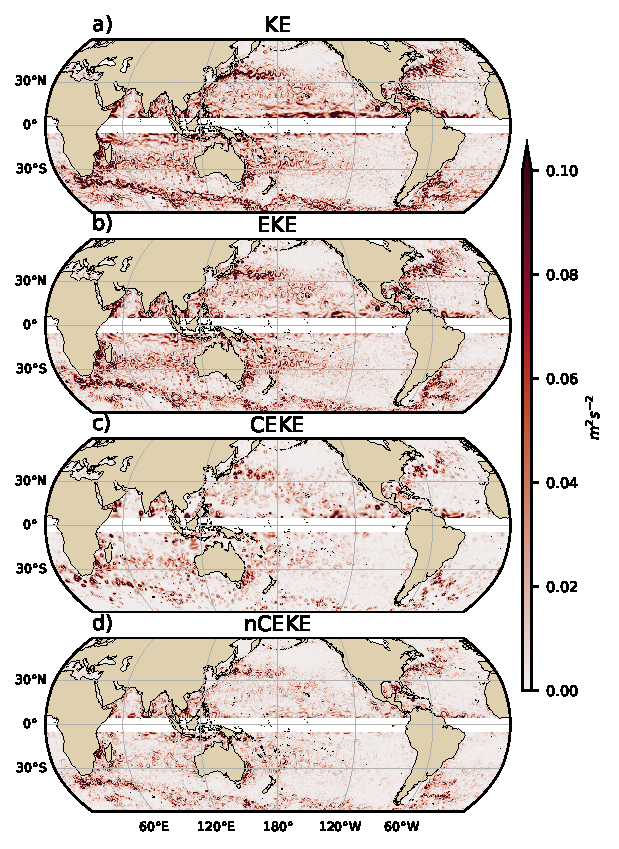
\includegraphics[width=95mm]{./figures/snapshot_ke_maps_satellite_large.pdf}
	    \caption{Snapshot of surface kinetic energy ($\KE$), surface eddy kinetic energy ($\EKE$), surface coherent eddy kinetic energy ($\CEKE$), and surface non-coherent eddy kinetic energy ($\nCEKE$) for the 1st of January 2017.}
	    \label{fig:eddy_snapshot}
	\end{figure}

	\subsection{Eddy statistics}

	The eddy statistics used in this study include (i) the eddy count ($\mathrm{cEddy}_{n}$) defined as the number of coherent eddies per grid cell, (ii) the eddy diameter defined as the diameter of a circle with equal area to the closed contour of each identified eddy, and (iii) the mean eddy amplitude defined as the mean amplitude of the coherent eddies within the cell ($\mathrm{cEddy}_{amp}$). The latter metric can be separated into positive ($\mathrm{cEddy}_{amp}^{+}$) and negative ($\mathrm{cEddy}_{amp}^{-}$) coherent eddy amplitudes, defined as the mean amplitude of warm core and cold core coherent eddies, respectively, within the cell. 
	The polarity independent eddy amplitude ($|\mathrm{cEddy}_{amp}|$) is defined as:
	\begin{equation}
	|\mathrm{cEddy}_{amp}| = \frac{1}{2} \left(\mathrm{cEddy}_{amp}^{+} -  \mathrm{cEddy}_{amp}^{-} \right)
	\end{equation}
	Note that the $\mathrm{cEddy}_{amp}^{+}$ and $\mathrm{cEddy}_{amp}^{-}$ are sign definite, thus the difference will always be positive, whereas the gridded averaged $\mathrm{cEddy}_{amp}$ can be negative or positive noting the dominant polarity of coherent eddies in the region, and the absolute value of $\mathrm{cEddy}_{amp}$ is denoted by $\mathrm{cEddy}_{|amp|}$.
	We analyze the climatology and trends of the above eddy statistics over the available satellite record, namely between 1993 and 2019. 
	We exclude the equatorial region (10$^\circ$S - 10$^\circ$N) and regions poleward of 60$^\circ$, because the geostrophic approximation is invalid near the Equator and the satellite spatial coverage at high-latitudes is unable to resolve the coherent eddy scales polewards of 60$^\circ$.
	Note that the climatology of $\mathrm{cEddy}_{n}$ is computed by adding all the identified eddies over the record, while all other climatological statistics are computed as the time-average over the record.  
	Seasonal climatologies are calculated for the monthly average of each coherent eddy statistic, while hemispheric time-series are filtered with a running average of 90 days. 
	Trends of $\mathrm{cEddy}_{n}$ and $|\mathrm{cEddy}_{amp}|$ are calculated by coarsening the dataset to a 5$^\circ$ grid, and then linear trends are computed for each grid point. The statistical significance of trends is assessed by a modified Mann-Kendall test above the 95\% confidence level \citep{Sheng_MK_2004}. 

	Time averages are denoted by $\overline{\phantom{X}}$, while area-weighted averages are denoted using $\left< \phantom{X}\right>$, where the area-weighted average of a function $f$ is:
	\begin{equation}
		\left< f \right>  = \frac{\int f \xi dx dy}{\int \xi dx dy},
	\end{equation}
	where $\xi$ is a mask that is set to zero in grid cells where no coherent eddies were identified and one elsewhere. 

	\section{Global Coherent Eddy Energetics}
	\label{sec:CEKE_climatology}


	The kinetic energy decomposition estimated from sea surface height measured by satellite altimeters averaged from 1993-2019 is shown in Figure \ref{fig:eddy_climatology}. 
	These maps show that many regions of the global ocean are highly energetic in mean KE ($\MKE$), mean EKE ($\MEKE$), mean coherent eddy kinetic energy ($\MCEKE$) and mean non-coherent eddy kinetic energy ($\MnCEKE$). 
	The spatial pattern highlights well-known regions of the ocean where mesoscale processes are abundant, such as the western boundary current (WBC) extensions and the Antarctic Circumpolar Current. 
	The spatial distribution of the energy contained by the reconstructed mesoscale coherent eddies and non-coherent components are similar (Figures \ref{fig:eddy_climatology}c,d). 
	However, there are some regions where coherent eddies dominate over non-coherent, and vice-versa. 
	Overall, this decomposition suggests that boundary current extensions and other energetic regions of the ocean contain both coherent and non-coherent components of the kinetic energy.

	\begin{figure}[t]
	    \centering
	    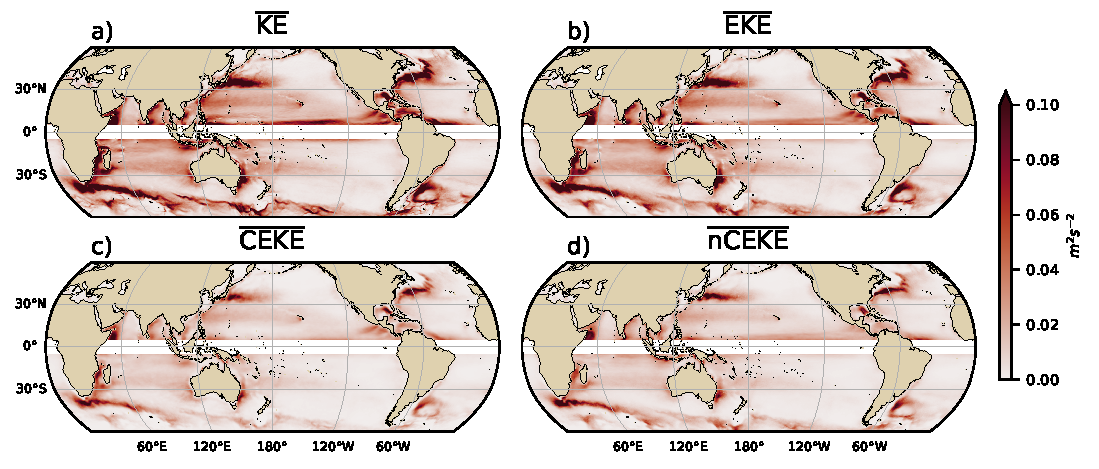
\includegraphics[width=1\textwidth]{./figures/mean_ke_maps_satellite.pdf}
	    \caption{a) Mean surface kinetic energy ($\MKE$); b) surface eddy kinetic energy ($\MEKE$); c) surface coherent eddy kinetic energy ($\MCEKE$), and d) surface non-coherent eddy kinetic energy ($\MnCEKE$) averaged between 1993-2018.}
	    \label{fig:eddy_climatology}
	\end{figure}


	\begin{figure}
	    \centering
	    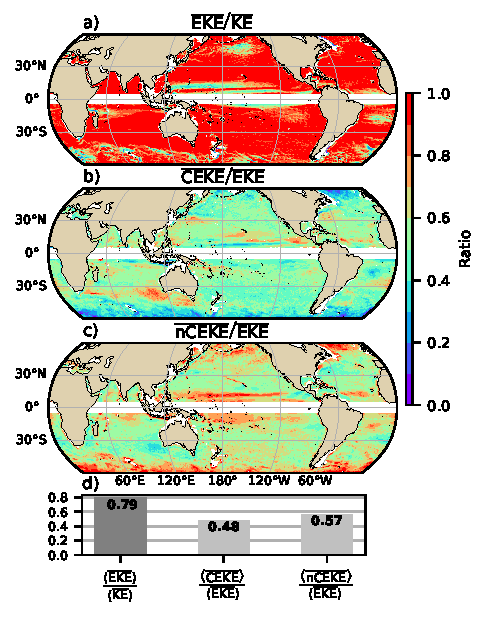
\includegraphics[width=1\textwidth]{./figures/eke_ratio_map_easy.pdf}
	    \caption{Ratios of the kinetic energy components. a) Map of the proportion of mean eddy kinetic energy ($\MEKE$) versus mean kinetic energy ($\MKE$);
		b) Map of the fraction of mean coherent eddy kinetic energy ($\MCEKE$) versus mean eddy kinetic energy ($\MEKE$);
		c) Map of the fraction of mean non-coherent eddy kinetic energy ($\MnCEKE$) versus mean eddy kinetic energy ($\MEKE$);
		d) Global time and area averaged (represented by $\left<\,\right>$) fraction of mean eddy kinetic energy ($\left<\MEKE\right>$) versus the global mean kinetic energy ($\left<\MKE\right>$), area averaged fraction of mean coherent eddy kinetic energy ($\left<\MCEKE\right>$) and mean non coherent eddy kinetic energy ($\left<\MnCEKE\right>$) versus global mean eddy kinetic energy ($\left<\MEKE\right>$). Regions where the depth of the ocean is shallower than 1000m are removed from the ratio estimation.
		}
	    \label{fig:eddy_ratio}
	\end{figure}

	Eddy kinetic energy is known to be more than an order of magnitude greater than kinetic energy of the mean flow ($\mKE$; \citealp{Gill_Energy_1974}); this result is clearly shown in Figure \ref{fig:eddy_ratio}a, which indicates that $\MEKE$ is responsible for almost all the $\MKE$ across the ocean, except for regions with persistent currents over time. 
	Such regions are located in the mean boundary extension locations, the equatorial Pacific currents and regions in the Antarctic Circumpolar Current, where the $\MEKE$ explains around 40\% of the $\MKE$. 
	In a previous study, \citet{Chelton_The_2011} estimated that coherent eddies with lifetimes greater than 4 weeks contain between 40-60\% of the $\MEKE$. 
	Our method to reconstruct the coherent eddy signature (Figure \ref{fig:eddy_ratio}b) further corroborates that the coherent eddy component ($\left<\MCEKE\right>$) has $\sim$48\% of the $\left<\MEKE\right>$ (Figure \ref{fig:eddy_ratio}d). 
	Furthermore, global area averages of the ratios show that $\left<\MEKE\right>$ explains $\sim$78\% of the ocean $\left<\MKE\right>$ field, while non coherent eddy features contain $\sim$57\% percent of the $\left<\MEKE\right>$. 
	Note that the globally averaged coherent and non coherent components do not add to 100\% as the cross terms ($\mathcal{O}_c^2$) are non-zero.
	The spatial pattern reveals a dominance of the $\MCEKE$ equatorward from the boundary current extensions and in areas with large coherent eddy contributions of around 80\% of the region's eddy kinetic energy, such as south of Australia, in the Tehuantepec Gulf, and in the tropical Atlantic. 
	An evident signal is a reduction of the energy contained by coherent eddies at high latitudes and an increase in the energy explained by non-coherent eddies; this signal could be a consequence of the inability of the 0.25$^\circ$ satellite resolution ($\sim$ 13 km at 60$^\circ$ latitude) to resolve coherent eddies with scales smaller than $\sim$10 km (first baroclinic Rossby radius at 60$^\circ$; \citealp{Chelton_Geographical_1998}).

	Figure \ref{fig:eddy_energy_polar} shows the seasonal cycle of the area-weighted $\EKE$ and $\CEKE$ for the Northern Hemisphere ($\left< \EKE\right>_{NH}$ and $\left< \CEKE\right>_{NH}$; 10$^\circ$N - 60$^\circ$N) and Southern Hemisphere ($\left< \EKE\right>_{SH}$  and $\left< \CEKE\right>_{SH}$; 60$^\circ$S - 10$^\circ$S). 
	In both hemispheres, the $\left<\EKE\right>$ and $\left<\CEKE\right>$ peak during summer. In the Northern Hemisphere, the largest $\left<\EKE\right>_{NH}$ and $\left<\CEKE\right>_{NH}$ occurs in July, $\sim$6 months after the maximum winds in January (purple bar and black star in Figure \ref{fig:eddy_energy_polar}c and d). Meanwhile, the Southern Ocean 
	$\left<\EKE\right>_{SH}$ and $\left<\CEKE\right>_{SH}$ seasonal maxima arise during December, $\sim$4 months after the maximum winds in August (purple bar and back star in Figure \ref{fig:eddy_energy_polar}g, and h). This lag between winds and the eddy and coherent eddy energy components is further discussed in Section \ref{sec:CE_stats}.

	The cyclic plots in Figure \ref{fig:eddy_energy_polar} show the temporal evolution of $\left<\EKE\right>$ and $\left<\CEKE\right>$. 
	Note that high frequency variability can be observed in the $\left<\CEKE\right>$ field with temporal scales of a few months, this variability could be attributed to regional dynamics averaged over the hemisphere (boundary currents, ocean gyres, etc.), as well as errors within the coherent eddy reconstruction. 
	% This signature will be further explored in section \ref{sec:CE_regional_stats}.
	Additionally, concentric changes in the cyclic plots highlight long-term changes over the record. For example, the Northern Hemisphere winters during early years of the record (blue) had a more energetic coherent eddy field, which has transitioned to weaker coherent energy content since 2010 (red), in other words, the intensity of the $\left<\CEKE\right>_{NH}$ field has decreased. A larger long-term change can be observed in the Southern Hemisphere, where concentric growth over time in $\left<\EKE\right>_{SH}$ and $\left<\CEKE\right>_{SH}$ supports the previously observed strengthening of the eddy field in the Southern Ocean \citep{Hogg_Recent_2015,Martinez_TKE_2019,Martinez_Kinetic_2021}. 

	\begin{figure}
	    \centering
	    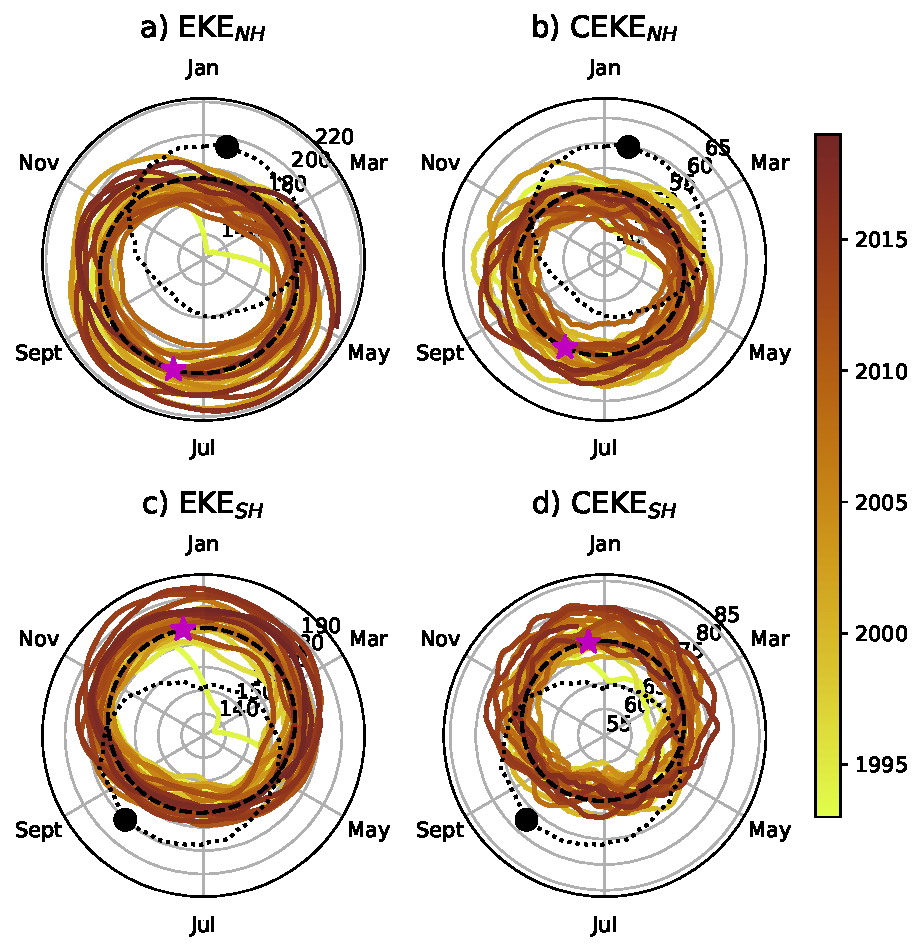
\includegraphics[width=95mm]{./figures/All_polar_plots.pdf}
	    \caption{Seasonality of the area-weighted eddy kinetic energy ($\left<\EKE\right>$) and coherent eddy kinetic energy ($\left<\CEKE\right>$). 
		Panels a) and b) show the time-series of the Northern Hemisphere, while panels e) and f) correspond to the Southern Hemisphere. Panels c) and d) show the seasonal cycle of the $\left<\EKE\right>_{NH}$ and $\left<\CEKE\right>_{NH}$ in the Northern Hemisphere, and panels g) and h) show the Southern Hemisphere ($\left<\EKE\right>_{SH}$ and $\left<\CEKE\right>_{SH}$).
		Bars correspond to the seasonal cycle of the fields and dotted lines show the seasonal cycle of the wind magnitude smoothed over 120 days (moving average). 
		The black stars and magenta markers (circle and bar) show the maximum of the seasonal cycle for the kinetic energy components and the wind magnitude, respectively. In the cyclic plots, line colors shows the year.}
	    \label{fig:eddy_energy_polar}
	\end{figure}
	
	\section{Global Coherent Eddy Statistics}
	\label{sec:CE_stats}

	Coherent eddy kinetic energy allows us to quantify and study the energy of the eddy field, but the coherent eddy properties computed by automated coherent eddy identification algorithms allow us to further investigate the contribution and temporal changes of their abundance (i.e. the number of eddies) and their intensity (both their amplitude and diameter). 
	Figure \ref{fig:eddy_stats_climatology} shows gridded estimates of the number of eddies and the eddy amplitude. 
	In this analysis, we contrast our MM19 eddy count with that of CS13 (\citealp{Chelton_Global_2007}; Figure \ref{fig:eddy_stats_climatology}a-b). Although the number of identified eddies is larger in MM19, possibly due to the lifespan filter implemented by CS13, both datasets reveal consistent spatial patterns. 
	For example, both datasets show an important meridional variation in the abundance of eddies, with high numbers of eddies in mid-latitudes and fewer eddies in the tropics and at high-latitudes ($\sim$60$^\circ$). Additionally, there is a tendency at mid-latitudes (30$^\circ$) for higher numbers of eddies in the eastern side of ocean basins (e.g. the East North Pacific, East North Atlantic, East South Pacific, and East South Atlantic). 
	Another interesting pattern emerges in both eddy count datasets, where small scale structures appear in the eddy count field. 
	These small structures highlight preferred coherent eddy paths observable in boundary current extensions and over regions of the Southern Ocean. 
	These structures and paths of coherent eddies could be associated with topographic features, with overall consistency between the eddy count patterns using the two different eddy identification methods.
	
	\begin{figure}
	    \centering
	    \includegraphics[width=1\textwidth]{./figures/global_stats_V1.pdf}
	    \caption{Averaged coherent eddy statistics. a) Climatology of the number of coherent eddies ($\cEddy_n$) identified by \citet{Chelton_Global_2007};  b) Climatology of the number of coherent eddies ($\cEddy_n$) identified by \citet{Martinez_TKE_2019}; c) Climatology of the mean absolute coherent eddy amplitude ($\cEddy_{amp}$), and d) Climatology of the mean coherent eddy amplitude ($\cEddy_{amp}$).}
	    \label{fig:eddy_stats_climatology}
	\end{figure}
	
	Regions with large counts of eddies have, in general, small absolute amplitudes (Figure \ref{fig:eddy_stats_climatology}c), for example, the eastern side of mid-latitude ocean basins.
	The ocean gyre interiors have a larger absolute amplitude and finally regions such as the boundary current extensions and the Antarctic Circumpolar Current have the largest coherent eddy absolute amplitudes, as also shown by \citet{Chelton_The_2011}.
	Eddy amplitude highlights regions dominated by a given coherent eddy polarity, for example, boundary current extensions have a preferred sign (Figure \ref{fig:eddy_stats_climatology} d); namely, positive amplitude polewards of the boundary current extension mean location, and negative amplitude equatorwards. 
	This sign preference is consistent with the preferential way that coherent eddies are shed from boundary current extensions; with warm core eddies (positive)  polewards of the boundary current extension, and equatorward for cold core eddies (negative) \citep{Chelton_Global_2007,Chelton_The_2011,Kang_eddy_characteristics_2013}. 
	These global statistics reveal the absolute coherent eddy amplitude as a proxy for the $\CEKE$ with similar spatial patterns (Figure \ref{fig:eddy_climatology} \& Figure \ref{fig:eddy_stats_climatology}c) and showcases that in regions where $\MCEKE$ accounts for a large proportion of $\MEKE$ (Figure \ref{fig:eddy_ratio}), the absolute coherent eddy amplitude is also large.

	To further understand the seasonal cycle of $\left<\CEKE\right>$, we compute the climatology of coherent eddy properties in each hemisphere (Figure \ref{fig:eddy_stats}). 
	The seasonality of the number of eddies in the Northern Hemisphere peaks in April (Figure \ref{fig:eddy_stats}a, c), while the Southern Hemisphere maximum number of eddies occurs during October (Figure \ref{fig:eddy_stats}e, g). 
	Meanwhile, the seasonality of the eddy amplitude ($\left<|\cEddy_{amp}|\right>$) peaks in August and January for the Northern and Southern Hemispheres respectively (Figure \ref{fig:eddy_stats}b, d, f, and h). 
	As expected, the seasonality of $\left<|\cEddy_{amp}|\right>$, equivalent to the intensity of the coherent eddies, is consistent with the seasonal cycle of $\left<\CEKE\right>$.

	A key feature of Figure \ref{fig:eddy_stats} is a distinct lag of $\sim$3 months between the winds and eddy count, while the eddy amplitude maximum occurs $\sim$6 months after the seasonal maximum in winds. 
	We suggest that the eddy number increases earlier in the year and, through eddy-eddy interactions (merging of coherent eddies), the coherent eddy amplitude increases $\sim$3 months after. This seasonal lag and summer maximum is consistent with previous studies which suggest that a time-lag of the inverse cascade \citep{Sasaki_seasonal_2014, Qiu_seasonal_2014} is responsible for the $\EKE$ seasonal cycle, where winter has the highest energy at the smallest scales (non-resolvable with satellite observations), spring and autumn have the highest and lowest energy at scales of 50-100 km, and summertime has the highest energy at the largest scales ($>$ 100 km; \citealp{Uchida_Seasonality_2017}). 
	Thus, the maximum of $\left<\EKE\right>$, $\left<\CEKE\right>$, and $\left<|\cEddy_{amp}|\right>$ located during summertime suggests that the seasonality of eddies and coherent eddies could be dominated by scales larger than 100 km.

	This result can be further explored by looking at the seasonal evolution of the eddy diameter ($\cEddy_d$). 
	Note that 90\% of identified coherent eddies have diameters between 50 and 220 km (Figure \ref{fig:eddy_diameter}a). We partition eddies into large-scale coherent eddies (diameter $>$ 120 km) and  small-scale coherent eddies (diameter $<$ 120 km; Figure \ref{fig:eddy_diameter}a). 
	In the Northern Hemisphere, small-scale eddies have a seasonal peak in diameter during May, while large-scale eddies have the greatest diameter in September (Figure \ref{fig:eddy_diameter}b).
	Meanwhile, in the Southern Hemisphere, the small-scale coherent eddies exhibit maximum diameter in December, while the diameter of large-scale coherent eddies peaks in February (Figure \ref{fig:eddy_diameter}~c). 
	This result suggests that wind driven baroclinic instabilities generate small coherent eddies early in the season, which then merge and grow to become larger in diameter and amplitude, and thus, more energetic. 
	This process is likely associated with the inverse energy cascade, and suggests that this mechanism not only drives $\EKE$ seasonality, but also may be responsible for the seasonal cycle of coherent eddies. 

	\begin{figure}
	    \centering
	    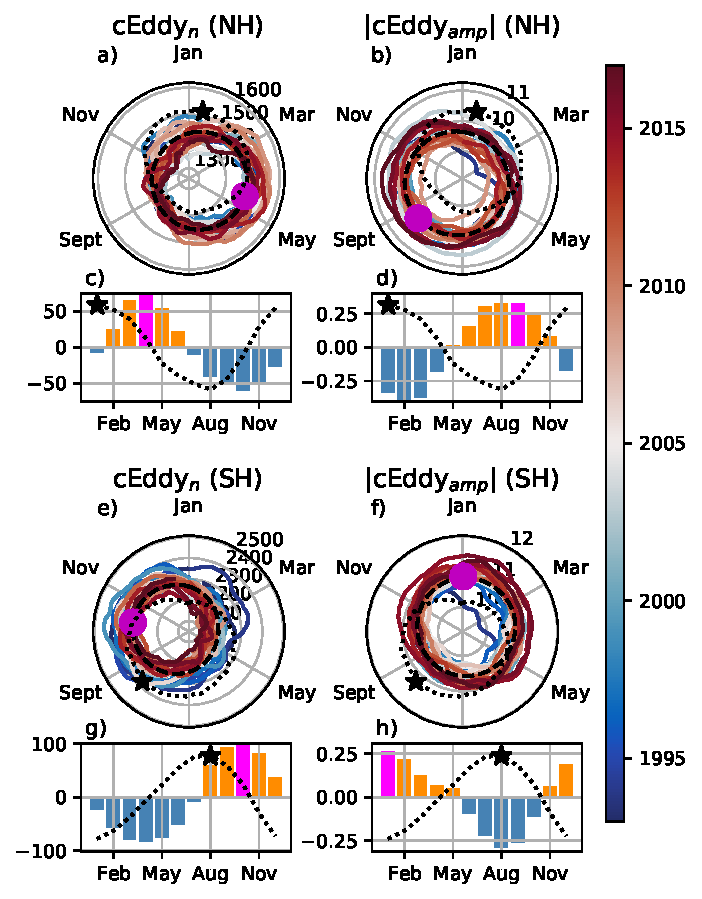
\includegraphics[width=95mm]{./figures/All_polar_plots_eddy_stats_polarity_V3.pdf}
	    \caption{
		Seasonality of the count of number of eddies ($\cEddy
		_n$) and the area-weighted polarity independent coherent eddy amplitude ($\left<\cEddy_{amp}\right>$); Panels a and b show the time-series of the Northern Hemisphere, while panels e and f correspond to the Southern Hemisphere. Panels c and d show the seasonal cycle of $\cEddy_n$ and $\left<|\cEddy|_{amp}\right>_{NH}$ in the Northern Hemisphere, and panels g and h show the Southern Hemisphere, $\cEddy_n$ and $\left<|\cEddy|_{amp}\right>_{SH}$.
		Bars correspond to the seasonal cycle of the fields and dotted lines show the seasonal cycle of the wind magnitude, smoothed over 120 days (moving average). 
		The black stars and magenta markers (circle and bar) indicate the maximum of the seasonal cycle for the eddy property, and the wind magnitude, respectively. In the cyclic plots, line color show the year from 1993-2019.}
	    \label{fig:eddy_stats}
	\end{figure}

	\begin{figure}
	    \centering
	    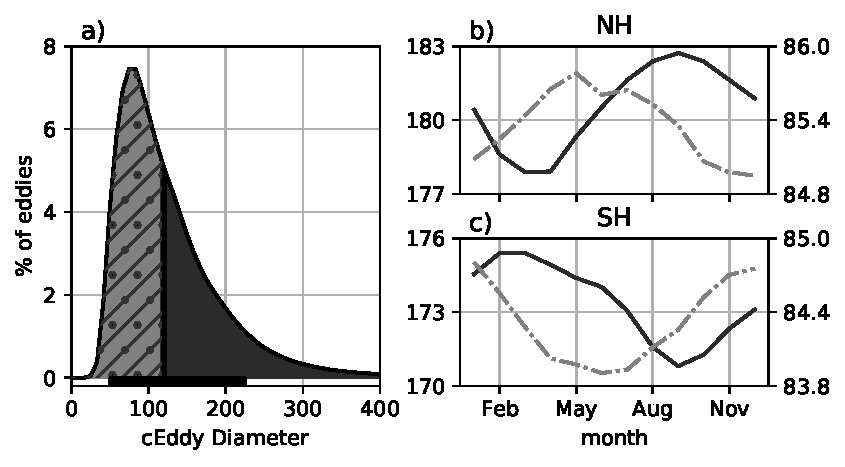
\includegraphics[width=1\textwidth]{./figures/eddy_diameter_seasonal.pdf}
	    \caption{Distribution of the identified eddy diameter ($\cEddy_d$; km) and hemispherical seasonality of the coherent eddy diameter. a) Distribution in percentage of identified eddy amplitude, solid bar below distribution represents 90\% of the identified eddies. Seasonal cycle of the eddy diameter for the b) Northern Hemisphere and c) Southern Hemisphere. Dark solid line and area corresponds to coherent eddies with diameters larger than 120 km, while light gray dash-dotted line and area shows coherent eddies with diameters smaller than 120 km.}
	    \label{fig:eddy_diameter}
	\end{figure}

	Long-term changes can be observed in Figure \ref{fig:eddy_stats}a,b, e, and f where growing/shrinking concentric circles over time denote an trend of the field. 
	This trend is particularly evident in the Southern Hemisphere, where the number of eddies has decreased, while the eddy amplitude has increased. 
	This result is consistent with the observed trends in $\EKE$ and mesoscale $\EKE$ in the Southern Ocean \citep{Hogg_Recent_2015, Martinez_TKE_2019}. The coherent eddy amplitude from positive coherent eddies and negative coherent eddies show similar seasonal cycles to the absolute eddy amplitude. The Northern Hemisphere decrease in absolute eddy amplitude is driven by a decrease of the amplitude of negative coherent eddies in the Northern Hemisphere. Meanwhile in the Southern Ocean, the increase in absolute eddy amplitude is corroborated by a strengthening of both coherent eddy polarities since the early 90s.

	\section{Trends}
	\label{sec:CE_trends}	
	
	The results presented in Figures \ref{fig:eddy_energy_polar} and \ref{fig:eddy_stats} suggest a long-term readjustment of the coherent eddy field. 
	The long-term trends of the number of coherent eddies, absolute coherent eddy amplitude, and coherent eddy amplitude polarities are further explored in Figure \ref{fig:eddy_stats_trends} contrasting the MM19 and CS13 methods. 
	Both MM19 and CS13 datasets show consistent spatial patterns in the trends and significance of the number of coherent eddies and the absolute coherent eddy amplitude. 
	Several regions in the ocean, such as the Southern Ocean, North Atlantic and North Pacific, show a decrease in the number of eddies. Those same regions also have a clear increase in the absolute coherent eddy amplitude. 
	These trends are similar to those observed in mesoscale eddy kinetic energy \citep{Martinez_Kinetic_2021} and provide additional evidence of a readjustment of the mesoscale eddy field over the last 3 decades. 

	The observed trends of $\cEddy_{|amp|}$ in several oceanic regions have the same scale as sea level rise ($\sim$3cm per decade). By analyzing the positive and negative coherent eddy amplitude, we filter out the observed trends that come from a net increase in sea level. 
	In fact, each coherent eddy polarity has intensified in the Southern Ocean and North East Pacific and Atlantic. 
	In other words, the amplitude of each polarity has increased over time, and thus this strengthening is an intrinsic response of the coherent eddy field. Note that the negative coherent eddy amplitude dominates the global $|\cEddy_{amp}|$ trends (Figure \ref{fig:eddy_stats_trends}e, f). However, different trend patterns can be observed in both positive and negative coherent eddy amplitudes in the North Atlantic and North Pacific, where the negative coherent eddy amplitude in the  Western Boundary Currents appears to decrease.

	\begin{figure}
	    \centering
	    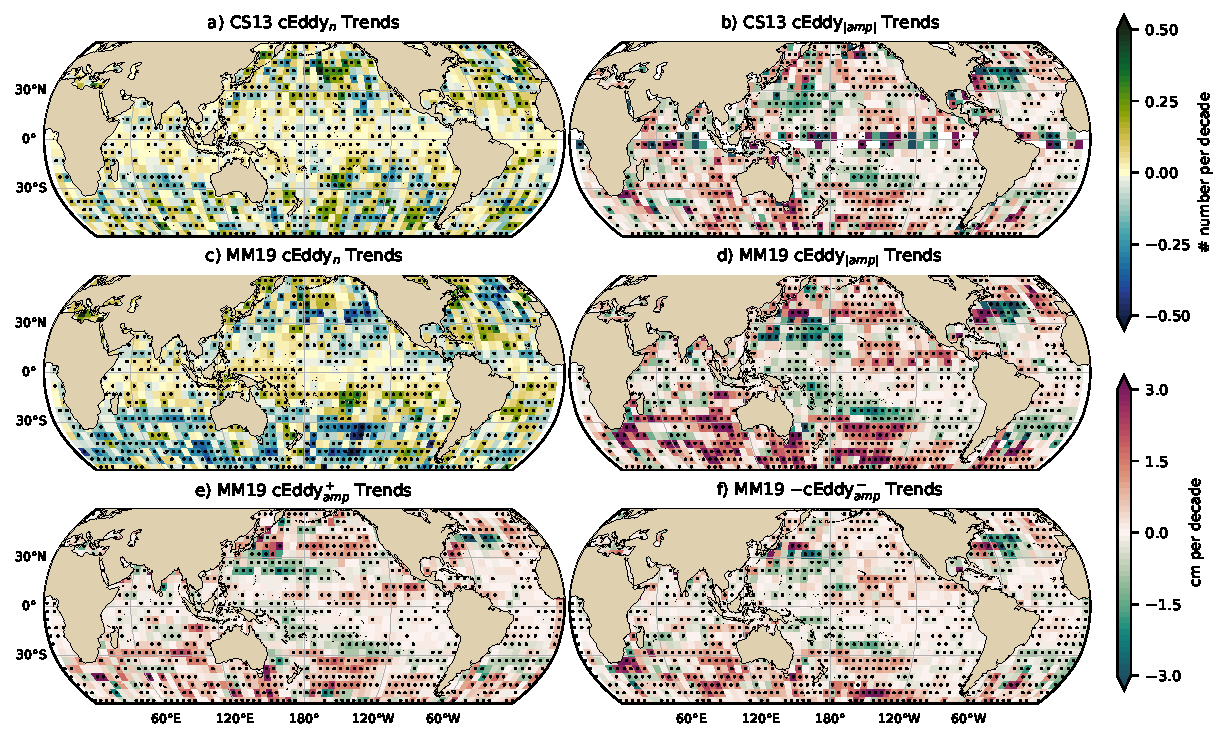
\includegraphics[width=1\textwidth]{./figures/all_trackeddy_trends_all_regular.pdf}
	    \caption{Trends of coherent eddy statistics. a) and c) Trends of the number of identified coherent eddies from satellite observations identified reported in CS13's dataset and using the TrackEddy scheme of MM19. b) and d) Trends of the absolute value of identified coherent eddy amplitude ($\cEddy_{|amp|}$) from satellite observations reported by CS13 and TrackEddy (after MM19). e) and f) Trends of the eddy amplitude polarity using TrackEddy ($\cEddy_{amp}^+$ and $\cEddy_{amp}^-$). Gray stippling shows regions that are statistically significant above the 95\% confidence level.}
	    \label{fig:eddy_stats_trends}
	\end{figure}


	\section{Regional Climatology}
	\label{sec:CE_regional_stats}
	
	For regions with relatively large proportions of $\CEKE$ located at WBC extensions and eastern boundary currents, we investigate the seasonal and long-term variability of the coherent eddy properties. The most energetic WBCs include the Gulf Stream, the Kuroshio Current, and the Agulhas Current (Figures \ref{fig:Gulf_Stream}, \ref{fig:Kuroshio}, and \ref{fig:Agulhas}). 
	Coherent eddy generation in boundary current extensions occurs through baroclinic and barotropic instabilities of the mean current, thus all these regions share similar generation dynamics. 
	In all these regions without exception; (i) $\CEKE$ contains 50-80\% of the $\EKE$ in regions equatorward from the mean WBC extensions, (ii) the number of eddies is consistently small over the mean WBC extensions, and (iii) the eddy amplitude is larger over the mean WBC extensions. 

	In the Gulf Stream, the energy ratio between $\CEKE$ and $\EKE$ is $\sim$56\% (Figure \ref{fig:Gulf_Stream}). 
	The highest energy ratio occurs in regions with numerous eddies, colocated with regions where the largest $|\cEddy_{amp}|$ gradients occur. 
	The time series of $\cEddy_{n}$ and $\left<|\cEddy_{amp}|\right>$ are anti-correlated (-0.52), and they display interannual and seasonal variability. 
	Although \citet{Chaudhuri_Oscillation_2009} observed that a positive phase of the North Atlantic Oscillation (NAO) exhibits higher $\EKE$, due to an increase in baroclinic instability, thus suggesting more coherent eddies, we do not find a correlation between the $\cEddy_{n}$ or the $\left<|\cEddy_{amp}|\right>$ in the Gulf Stream and the NAO index. 
	Similar to the signal observed in the hemispheric analysis, the eddy count seasonal cycle follows the wind maximum lagging by $\sim$3 months, while the amplitude of the coherent eddies lags by $\sim$ 6 months. 

	\begin{figure}
	    \centering
	    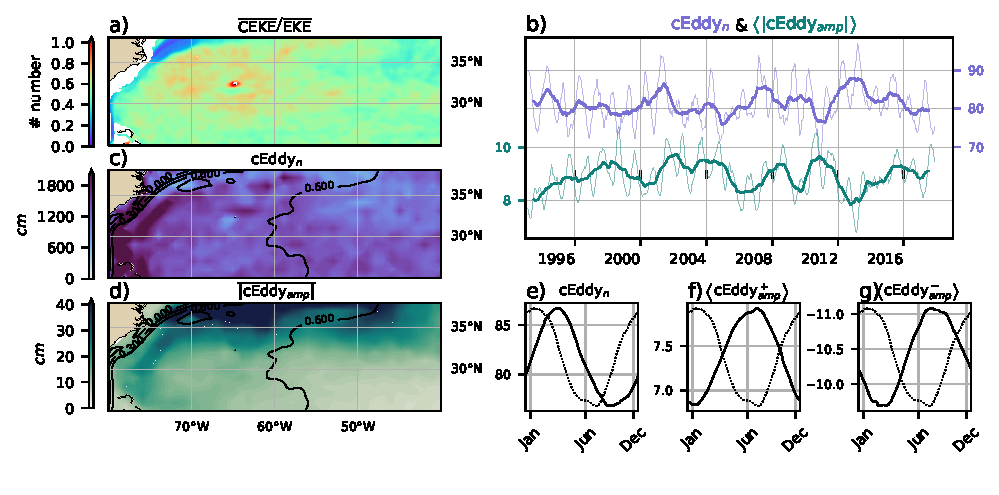
\includegraphics[width=1\textwidth]{./figures/regional_ratios_and_stats_V3_5.pdf}
	    \caption{Climatology of the eddy field and coherent eddy field in the Gulf Stream. a) Ratio of mean coherent eddy kinetic energy ($\MCEKE$) versus mean eddy kinetic energy ($\MEKE$); b) Thick lines show the running average over 2 years and thin lines show the running average over 90 days of the coherent eddy number sum and the average coherent eddy amplitude; c) Map of the number of eddies; d) Map of the average coherent eddy amplitude; e) Seasonal cycle of the number of eddies ($\cEddy_n$); f) Seasonal cycle of the positive coherent eddy amplitude ($\left<\cEddy_{amp}^+\right>$), and g) Seasonal cycle of the negative coherent eddy amplitude ($\left<\cEddy_{amp}^-\right>$). Contours in maps correspond to mean sea surface height (m). Dotted lines show the seasonal cycle of the wind magnitude.}
	    \label{fig:Gulf_Stream}
	\end{figure}

	The variability of the $\cEddy_{n}$ and $\left<|\cEddy_{amp}|\right>$ in the Kuroshio Current are weakly anti-correlated (-0.41; Figure \ref{fig:Kuroshio}). 
	However, on average 56\% of the energy in the region corresponds to $\CEKE$.
	As observed in the Gulf Stream, there is an important seasonal cycle in the boundary current extension, where the eddy count seasonal cycle peak occurs in March, lagging the wind maximum by $\sim$3 months (January). Meanwhile, the amplitude of the coherent eddies lags the wind maximum by $\sim$ 6 months (June). 

	\begin{figure}
	    \centering
	    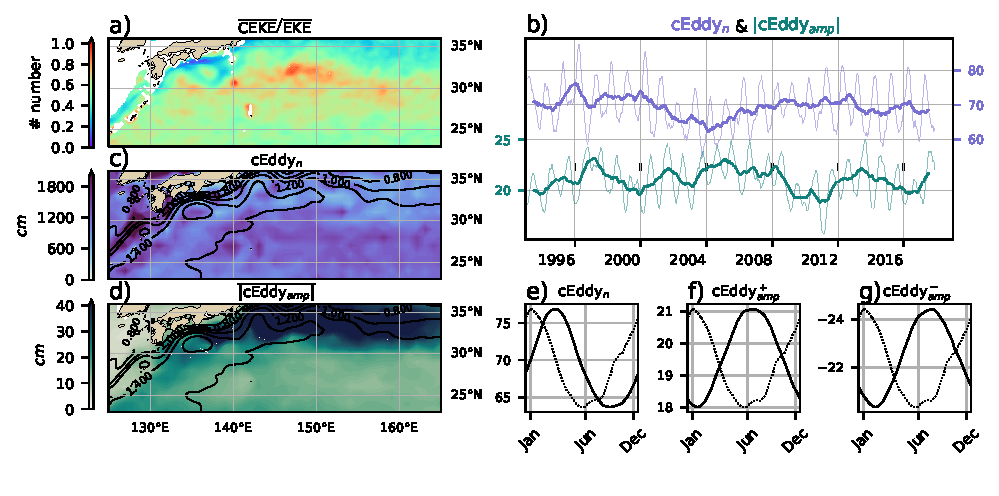
\includegraphics[width=1\textwidth]{./figures/regional_ratios_and_stats_V3_4.pdf}
	    \caption{As in Figure \ref{fig:Gulf_Stream}, only showing the climatology of the eddy field and coherent eddy field in the Kuroshio extension. a) Ratio of mean coherent eddy kinetic energy ($\MCEKE$) versus mean eddy kinetic energy ($\MEKE$); b) Time-series of the coherent eddy number and the average coherent eddy amplitude; c) Map of the number of eddies; d) Map of the average coherent eddy amplitude; Seasonal cycle of the e) number of eddies; f) positive coherent eddy amplitude, and g) negative coherent eddy amplitude.}
	    \label{fig:Kuroshio}
	\end{figure}

	In the Southern Hemisphere the strongest boundary current, the Agulhas Current, shows similar behavior to its counterparts in the Northern Hemisphere (Figure \ref{fig:Agulhas}). On average, coherent eddies in the Agulhas Current contain $\sim$56\% of the energy, meanwhile the $\cEddy_{n}$ seasonal peak occurs in August, while the $\left<|\cEddy_{amp}|\right>$ peak occurs in January-February. 
	The seasonal lag between the winds, eddy count, and eddy amplitude in each of the WBC extensions is interpreted as being analogous to the lagged response of coherent eddy properties (Figure \ref{fig:eddy_stats}) due to eddy-eddy interactions, consistent with the inverse cascade of energy.

	\begin{figure}
	    \centering
	    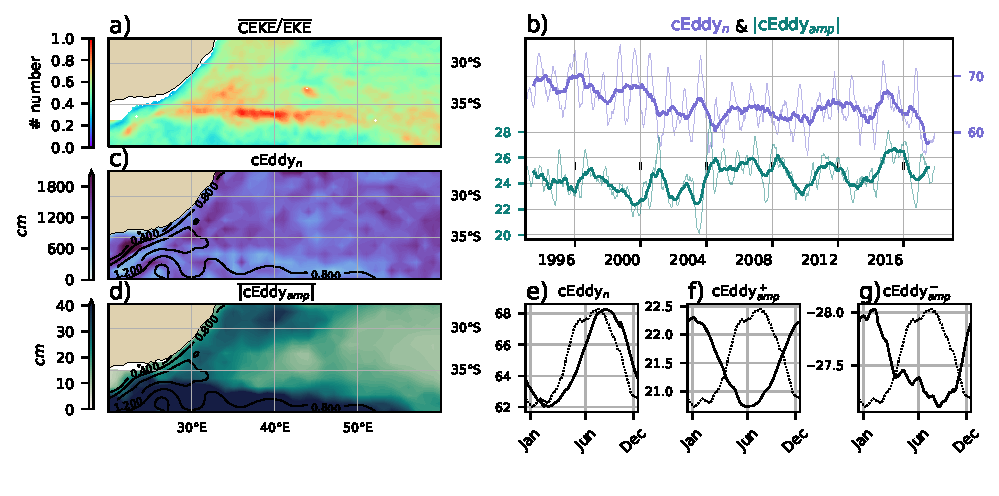
\includegraphics[width=1\textwidth]{./figures/regional_ratios_and_stats_V3_2.pdf}
	    \caption{As in Figure \ref{fig:Gulf_Stream}, only showing the  climatology of the eddy field and coherent eddy field in the Agulhas Current. a) Ratio of mean coherent eddy kinetic energy ($\MCEKE$) versus mean eddy kinetic energy ($\MEKE$); b) Time-series of the coherent eddy number and the average coherent eddy amplitude; c) Map of the number of eddies; d) Map of the average coherent eddy amplitude; Seasonal cycle of the e) number of eddies; f) positive coherent eddy amplitude, and g) negative coherent eddy amplitude.}
	    \label{fig:Agulhas}
	\end{figure}

	Coherent eddies dominate the $\EKE$ field in other regions such as the Leeuwin Current (Figure \ref{fig:leeuwin_cycle}), where 65\% of the energy is contained in coherent eddies. 
	The Leeuwin region is not characterized by having a large $\EKE$, however, a considerable abundance of eddies and large eddy amplitudes are observed in the region. 
	The time-series reveal a significant increase in the $\left<|\cEddy_{amp}|\right>$, while the $\cEddy_{n}$ has decreased over the last 3 decades. 
	The seasonal cycle shows that the $\cEddy_{n}$ peak occurs in August, 3 months after the maximum winds (June). 
	Meanwhile, the $\left<\cEddy_{amp}^+\right>$ responds in synchrony to the winds, and the $\left<\cEddy_{amp}^-\right>$ is in phase with the seasonal cycle of the eddy number ($\cEddy_{n}$). 
	Hence, this region contrasts with the behavior of WBC extensions, and showcases the spatial variability of the seasonal cycle of coherent eddies.
 		
	
	\begin{figure}
	    \centering
	    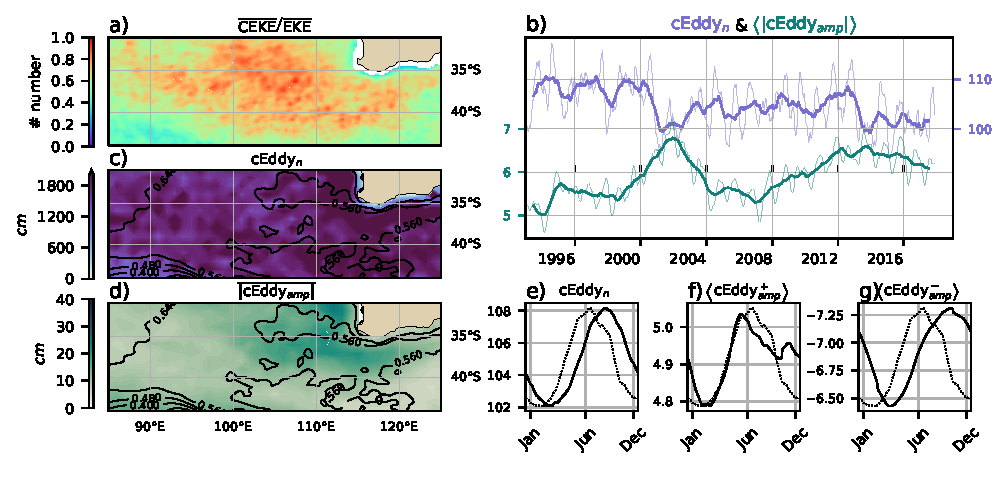
\includegraphics[width=1\textwidth]{./figures/regional_ratios_and_stats_V3_0.pdf}
	    \caption{As in Figure \ref{fig:Gulf_Stream}, only showing the  climatology of the eddy field and coherent eddy field in the Leeuwin Current. a) Ratio of mean coherent eddy kinetic energy ($\MCEKE$) versus mean eddy kinetic energy ($\MEKE$); b) Time-series of the coherent eddy number and the average coherent eddy amplitude; c) Map of the number of eddies; d) Map of the average coherent eddy amplitude; Seasonal cycle of the e) number of eddies; f) positive coherent eddy amplitude, and g) negative coherent eddy amplitude.}
	    \label{fig:leeuwin_cycle}
	\end{figure}

	Another region with important contributions to the coherent eddy field is the East Tropical Pacific (Tehuantepec region; Figure \ref{fig:tehuantepec}), where coherent eddies contain $\sim$58\% of the energy. 
	In fact, coherent eddy generation in this region is modulated by winds and coastally trapped waves which produce a strong horizontal and vertical shear (baroclinic and barotropic instabilities; \citealp{Zamudio_Tehuantepec_2006}). 
	Furthermore, the equatorial generated waves propagating along the coast have an important interannual variability observable in the $\left<|\cEddy_{amp}|\right>$ time-series, where El Niño events are notable during 1997 and 2015 (Figure \ref{fig:tehuantepec}b). 
	The seasonal cycle of $\cEddy_{n}$, $\left<\cEddy_{amp}^+\right>$, and $\left<\cEddy_{amp}^-\right>$ support the idea of a coherent eddy response to two different coherent eddy generation mechanisms; the number of eddies lags by $\sim$3 months from the winds, while the $\left<\cEddy_{amp}^+\right>$ is in phase with the winds and the time of maximum trapped wave activity (winter; \citealp{Zamudio_Tehuantepec_2006}), while the $\left<\cEddy_{amp}^-\right>$ could be a consequence of eddy-eddy interactions. 


	\begin{figure}
	    \centering
	    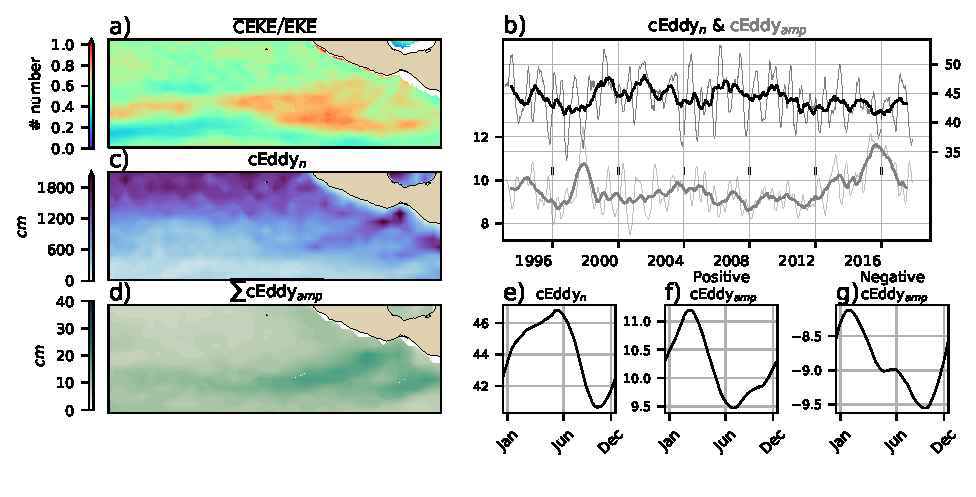
\includegraphics[width=1\textwidth]{./figures/regional_ratios_and_stats_V3_3.pdf}
	    \caption{As in Figure \ref{fig:Gulf_Stream}, only showing the  climatology of the eddy field and coherent eddy field in the East Tropical Pacific. a) Ratio of mean coherent eddy kinetic energy ($\MCEKE$) versus mean eddy kinetic energy ($\MEKE$); b) Time-series of the coherent eddy number and the average coherent eddy amplitude; c) Map of the number of eddies; d) Map of the average coherent eddy amplitude; Seasonal cycle of the e) number of eddies; f) positive coherent eddy amplitude, and g) negative coherent eddy amplitude.}
	    \label{fig:tehuantepec}
	\end{figure}	


	\section{Discussion and Conclusions}	
	\label{sec:Conclusions}

	We have investigated the contribution of coherent eddies to the total kinetic energy field using available satellite observations. 
	We found that around half of the $\EKE$ is explained by coherent eddies. 
	This half is concentrated in eddy-rich regions where a recent multi-decadal intensification of the eddy field has been observed \citep{Martinez_Kinetic_2021}. The energy contained by eddies is larger than the previous estimate of 40\% by \citet{Chelton_The_2011}.
	Although there are differences in the identification criteria of both eddy identification methods, the main cause of the difference is likely to be the lifespan and amplitude filters. 
	These filters are widely used to track individual eddies in space and time, however, interactions between eddies in energetic regions may obscure the abundance and influence of short-lived coherent eddies. 
	Filters are not used in this study, and indeed a lack of filters could facilitate an over-estimation of the the energy contained by coherent eddies, when mis-identifying or mis-fitting a coherent eddy. 

	It should also be noted that regions with first baroclinic Rossby radius of deformation smaller than 10km cannot be resolved by satellite observations. 
	Thus, the energy contained in coherent eddies around latitudes of 60$^\circ$ and those near the shore are missed from this estimate, and their role in the seasonal cycle and local dynamics remains unknown. New satellite altimeter missions (e.g. Surface Water and Ocean Topography; SWOT) may allow estimates of the energy contained in mesoscale coherent eddies outside the subtropical regions and over the continental slope.

	Hemisphere-wide variability indicates a strong seasonal cycle of the $\EKE$, $\CEKE$, and eddy properties. 
	The seasonal cycle of the $\CEKE$ in each hemisphere occurs as a consequence of numerous small coherent eddies interacting with each other (eddy-eddy interactions) and resulting in stronger, larger and more energetic (but fewer) coherent eddies during summer, a few months after the yearly coherent eddy number maximum.
	This result reveals eddy-eddy interactions and thus the transfer of energy from smaller coherent eddies to larger coherent eddies could explain the observed seasonal cycle of $\CEKE$ and coherent eddies properties.
	
	Coherent eddy properties reveal a non-uniform long-term readjustment of the mesoscale eddy field. 
	Overall, the eddy number has decreased globally at a significant rate of $\sim$35 eddies per decade from $\sim$4000 eddies identified globally on average each day. Despite the small changes in the total eddy numbers, large proportions of the ocean show a major strengthening of the mesoscale coherent eddy amplitude at rates greater than $\sim$1 cm per decade.
	This strengthening of the coherent eddy amplitude is attributed to an intensification of each coherent eddy polarity, rather than a readjustment of the coherent eddy field to sea level rise. 
	In other words, the coherent eddy amplitude intensification is occurring in both coherent eddy polarities and a proportion of the previously observed readjustments in the eddy field to long-term changes in the ocean forcing \citep{Hu_acceleration_2020,Wunsch_speeding_2020,Martinez_Kinetic_2021}. 
	This long-term readjustment reveals an intensification of the coherent eddy field, possibly due to long-term readjustments in the ocean baroclinic and barotropic instabilities, as well as the strength of the winds.
	
	The reconstruction of the coherent eddies and their statistics has revealed regions with important coherent eddy contributions and a distinct seasonal evolution of the coherent eddies. 
	Western boundary current (WBC) extensions generate eddies through the instability of the main currents and the seasonal cycle of coherent eddies, $\CEKE$, and thus $\EKE$ could be associated with an inverse energy cascade observable through lagged seasonal cycles in the coherent eddy statistics. 
	In addition, the amplitude of the seasonal cycle in WBC extensions is two times larger than any other region, thus the seasonality of the coherent eddies in WBC extensions dominates the hemispheric seasonal cycle. 
	Furthermore, the seasonal lag of the inverse energy cascade is coupled with the presence of fronts \citep{Qiu_seasonal_2014}, such as the case for WBC extensions, and our results are consistent with the notion of baroclinic instability generating eddies and, via eddy-eddy interactions, a lagged inverse energy cascade.
	
	The use of satellite observations in this study limits our ability to quantify the importance of the inverse energy cascade seasonality in the control of the coherent eddy seasonal cycle. 
	As mentioned above, there is robust evidence of an increase in eddy-eddy interactions, however we cannot discard important contributions from other processes such as the seasonal cycle of forcing, stratification, and instabilities, which are crucial in the generation of coherent eddies. Although this study can provide a descriptive response of the coherent eddy field, further work is needed to assess the role of eddy-eddy interactions in our changing climate, ocean dynamics, and biogeochemical processes. Furthermore, the SWOT mission could allow us to advance our understanding of eddy-eddy interactions and the seasonal cycle of scales smaller than mesoscale, which may provide further evidence of the inverse energy cascade driving the coherent eddy seasonality. Current generation climate models have just started to resolve mesoscale dynamics, thus, the presented estimate of energy in coherent eddies from satellite observations could be used as a benchmark that facilitates the evaluation of such models, and to quantify the energy contained by mesoscale and more specifically coherent eddies in future climate projections.

	\acknowledgments
	The \citet{Chelton_mesoscale_2013} dataset was produced by SSALTO/DUACS and distributed by AVISO+ (\url{https://www.aviso.altimetry.fr/}) with support from CNES, developed and validated in collaboration with E.Mason at IMEDEA.
	Global coherent eddy reconstruction, coherent and non-coherent eddy kinetic energy datasets, in addition to gridded coherent eddy tracking datasets are publicly available at (\url{https://doi.org/10.5281/zenodo.4646429}).
	All analyses and figures in this manuscript are reproducible via Jupyter notebooks and instructions can be found in the Github repository \texttt{CEKE\_climatology} (\url{https://github.com/josuemtzmo/CEKE_climatology}). Trends used the Python Package xarrayMannKendall (\url{https://doi.org/10.5281/zenodo.4458776}). J.M.-M. was supported by the Consejo Nacional de Ciencia y Tecnolog\'ia (CONACYT), Mexico funding. M.H.E. is supported by the Centre for Southern Hemisphere Oceans Research (CSHOR), a joint research centre between Qingdao National Laboratory for Marine Science and Technology (QNLM), Commonwealth Scientific and Industrial Research Organisation (CSIRO), University of New South Wales (UNSW), and the University of Tasmania (UTAS).  Analyses were undertaken on the National Computational Infrastructure in Canberra, Australia, which is supported by the Australian Commonwealth Government. 
	
	\bibliography{biblio.bib}
	
\end{document}
